\documentclass[10pt,conference,compsocconf,a4paper]{IEEEtran}

\usepackage{graphicx}
\usepackage{amsmath, amssymb}
\usepackage{commath}
\usepackage{booktabs}
\usepackage{siunitx}
\usepackage[labelformat=simple, labelfont=normalfont]{subcaption}  % Side-by-side figures
\usepackage[labelfont=sc]{caption}  % Using captionof outside of figure environment
\usepackage[colorlinks, bookmarks=false, citecolor=black, linkcolor=black, urlcolor=blue]{hyperref}  % Cite colors + autoref
\usepackage{xurl}  % hypen breaks in urls

\newcommand{\G}{\mathcal{G}}
\renewcommand{\vec}[1]{\boldsymbol{#1}}
\newcommand{\funit}[1]{\ [\si{#1}]}  % formula unit
\newcommand{\nunit}[1]{\ \si{#1}}  % numerical unit
\newcommand{\avg}[1]{\langle{#1}\rangle}

% braces around equation number in referencing
\makeatletter
\let\oldtheequation\theequation
\renewcommand\tagform@[1]{\maketag@@@{\ignorespaces#1\unskip\@@italiccorr}}
\renewcommand\theequation{(\oldtheequation)}
\makeatother

% Prevent latex from streching out paragraph spacings
\raggedbottom

% braces around subfig number
\renewcommand\thesubfigure{\,(\alph{subfigure})}

% Smallcaps short autoref
\newcommand*{\shortautoref}[1]{%
	\begingroup
	\def\equationautorefname{\textsc{Eq.}}%
	\def\tableautorefname{\textsc{Tab.}}%
	\def\figureautorefname{\textsc{Fig.}}%
	\autoref{#1}%
	\endgroup
}

% Itemize spacing
\let\olditemize=\itemize
\let\endolditemize=\enditemize
\renewenvironment{itemize}{\olditemize \itemsep0em}{\endolditemize}

% subfigure spacing
\captionsetup[subfigure]{aboveskip=1pt}

\begin{document}
\title{Convolutional graph neural networks for tracking yeast cells}

\author{
	G. Brenna, F. Massard, N. Vadot\\
	\textit{EPFL, Switzerland}
}

\maketitle

\begin{abstract}
	We present a graph-based machine learning method that is able to track yeast cells throughout a movie, after having segmented the frames (here, this is done with YeaZ \cite{dietler_convolutional_2020}). The method achieves better accuracy than the Hungarian algorithm implemented in YeaZ, thanks to the context-awareness of the graph structure. The method relies on translating the tracking problem to a binary node classification problem, and should generalize to any tracking problem where segmentations are available. The source code, as well as explicative Python notebooks, are available at \cite{vadot_cs-433_2021}.
\end{abstract}


\section{Context}

	The tracking problem emerges when addressing a more specific problem, that of lineage determination of budding yeast : for each new bud, the parent cell needs to be determined. This is made difficult in densely packed environments, but budneck markers can be used to manually determine the parent of each bud. However, it might not always be convenient to use such markers, and the question arises if lineage determination is possible with only a phase contrast image. Buds are most visible when they grow, so a machine learning algorithm might be able to pick up on spatio-temporal correlations in the segmentations to determine the parent. However, feeding a machine learning algorithm coherent temporal information requires a consistent tracking of the cells, which is the main problem this report addresses.

	The classical approach to tracking is to extract some features from the segmentation geometry (YeaZ uses cell surface area and center of mass), and minimize the pairwise euclidean distance in the feature space using the Hungarian algorithm. The problem with this method is that it starts to break down for large colonies, since in that regime many cells have similar geometry and entire sections of the colony might drift away. Then, it would be interesting to look at pairwise relationships between cells and their nearest neighbors to track the cells, similarly to how puzzle pieces fall into place given the right context.

	A graph-based approach arises, which can naturally encode cells as nodes with certain features, and nearest-neighbor relationships are edge features. The recent development of graph neural networks (GNN) \cite{zhou_graph_2021} and growing open-source codebase \cite{paszke_pytorch_2019, fey_fast_2019} makes it possible to easily implement machine learning methods that are able to learn on graphs.


\section{Prior work}

	The problem of tracking arises in other domains, such as reconstruction of particle trajectory in detectors \cite{dezoort_charged_2021}. In this approach, timestamped detection events in cylindrical coordinates are represented as nodes, and edge features are constructed by considering geometrical differences of the two detection events it connects. Features are then encoded with an MLP, and an edge-classification task is performed in order to attribute multiple detection events to the same particle. In our context, cells are not moving in a highly correlated manner like a particle through a detector, but the idea of encoding geometrical features can be repurposed.

	Tracking nodes, as they evolve in time-dependent graphs, can be reformulated as the problem of graph matching. \cite{kipf_semi-supervised_2017} considers the problem of finding a subgraph in a larger graph. It does this by applying graph convolutions, embedding the nodes in a high-dimensional space, and minimizing the total cost of pairwise euclidean distance to match nodes from the two graphs. We try to reformulate the tracking problem as a graph matching problem, and use a similar idea by maximizing a score to assign nodes between two graphs.

	% Other papers \cite{cordonnier_extrapolating_2019} propose a graph neural network-based approach to predict trajectories, however they assume highly correlated motion or decision agents responsible for the motion, which is not applicable here. Furthermore, the task here is to reconstruct trajectories, not to predict them.


\section{Data preprocessing} \label{sec:data_preprocessing}

	\subsection{Feature extraction and cell graph generation}

		The full data preprocessing pipeline is schematized in \shortautoref{fig:pipeline}. The data used here consists of 5 colonies of budding yeast, with phase contrast images taken at 5 minute intervals, for a total of 180 images (15 hours of growth time) per colony. The first 4 colonies (in the data, named \texttt{colony00[0123]}) are used for generating training (and validation) datasets, and the last colony (named \texttt{colony007}) is kept as a final testing set. On average, the colonies started with 2 cells and had 110 cells at the end.

		The movies were segmented and tracked semi-automatically using YeaZ \cite{dietler_convolutional_2020}. From the segmentation masks, simple geometrical features were extracted from the cells : surface area $A$, radius $r$ and eccentricity $e$. To do this, an ellipse was fitted to the cell by using PCA analysis on the cell mask coordinates, which can then be used to obtain the semi-major and minor axes $a$ and $b$ respectively. Then we compute $e=\sqrt{1-(\frac{a}{b})^2}$, and the radius of the circle with the same area as the ellipse $r=\sqrt{ab}$. \shortautoref{fig:hist_x} shows the distribution of the node features. The distributions are strongly peaked around their mean, respectively $\avg{A} \approx 21 \pm 14 \nunit{\micro \meter \squared}$, $\avg{r} \approx 2.5 \pm 0.8 \nunit{\micro \meter}$ and $\avg{e} \approx 0.52 \pm 0.14$. Notice the distribution for $r$ has a few outliers corresponding to very large cells, and these outliers are even more visible for $A$, explained by the scaling law $A \sim r^2$. It however doesn't make sense to remove these outliers, since that would have the same effect as removing the cell from the colony, impacting its direct neighbors.

		Nearest neighbor features were extracted by considering the contour of each cell mask, and placing an edge between cells if the minimum distance between their contours is below $1.3 \nunit{\micro \meter}$ (this threshold is arbitrary, and can be changed as needed when calling \texttt{bread\_nn.graph.build\_cellgraph}). Extracted features are $\rho$, the center of mass (CM) to CM distance between the neighboring cells, $\theta$, the angle of the CM to CM vector with respect to the horizontal axis, and $\ell$, the minimal distance between the contours. \shortautoref{fig:hist_e} shows the distribution of these features. $\rho$ shows a distribution peaked around $\avg{\rho} \approx 5.4 \pm 1.2$, which makes sense, as on average cell has a radius of $r \approx 2.5 \nunit{\micro \meter}$, meaning two average cells would be separated by approximately $2r \approx 5.0 \nunit{\micro \meter}$. $\theta$ shows a near-uniform distribution, with mean and standard deviation $\avg{\theta} \approx 0 \pm 1.8$. Again, this is intuitive, since we don't expect cells to be preferentially aligned in one direction. Note that we allow $\theta$ to take values in $[-\pi, \pi]$ instead of $[0, \pi]$, because edges are not stored bidirectionally (to save memory), so the sign of $\theta$ encodes directionality of the edge. $\ell$ is strongly peaked around $\avg{\ell} \approx 0.34 \pm 0.22 \nunit{\micro \meter}$. Physically, $\ell$ is not that representative since membranes are supposed to be in contact, and the mean being slightly offset is an artifact from the segmentation process. Nevertheless, $\ell$ can be a good distance metric between cells, since it is independent of their sizes.

		In total, 720 cell graphs we constructed, for a total of 25510 nodes and 48018 edges (note : edges are considered bidirectional, but are stored as one-directional to save memory). The Python notebook used for this process can be found under \texttt{experiment\_gnn/build\_cellgraphs.ipynb}.

	\subsection{Assignment graph generation}

		We formulate the tracking problem as a graph matching problem. Suppose we have generated two graphs $\G^{(1)}$ and $\G^{(2)}$ storing extracted features from two segmentations, and we want to track cells from segmentation (1) to segmentation (2). For this, we construct an assignment graph $\G^{(a;x,e)}$. Let $\vec{v_i^{(1)}}, \vec{e_{i,j}^{(1)}}$ (resp. $\vec{v_a^{(2)}}, \vec{e_{a,b}^{(1)}}$) encode the nodes and edges of $\G^{(1)}$ (resp. $\G^{(2)}$). Nodes $\vec{v_{ia}^{(a)}}$ of $\G^{(a;x,e)}$ are obtained by concatenating features from $\vec{v_i^{(1)}}$ and $\vec{v_a^{(2)}}$. Edges $\vec{e_{ia,jb}^{(a)}}$ of $\G^{(a)}$ link nodes $\vec{v_{ia}^{(a)}}$ and $\vec{v_{jb}^{(a)}}$ if $\vec{e_{i,j}^{(1)}}$ and $\vec{e_{a,b}^{(2)}}$ exist in $\G^{(1)}$ and $\G^{(2)}$ respectively, in which case edge features are similarly obtained by concatenation.

		Finally, we similarly build the corresponding target graph $\G^{(a;y)}$, where the node features are simply 2-dimensional one-hot encoder vectors, indicating whether a node $\vec{v_{ia}^{(a)}}$ corresponds to a correct tracking. Note that at this point, there is no trace left of the cell ids that were used to differentiate cells in the segmentations.

		Concretely, the assignment graph dataset was obtained by considering all pairs of segmentations separated by at most 20 frames (1h40), constructing the assignment graphs, and repeating this for each colony. The Python notebook used for this process can be found under \texttt{experiment\_gnn/build\_assgraphs.ipynb}.

		\begin{figure*}
			\centering
			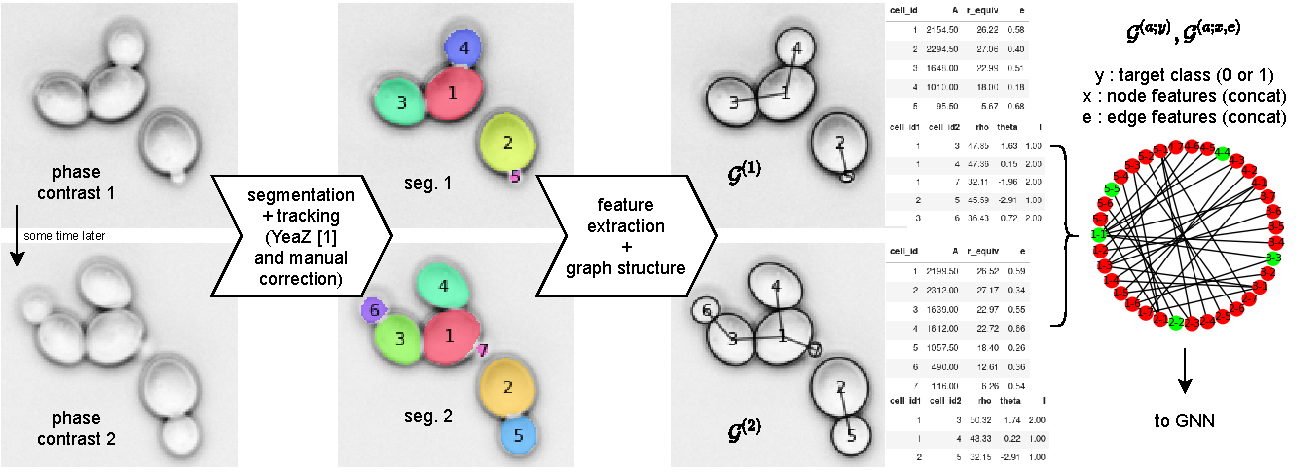
\includegraphics[width=\linewidth]{figures/pipeline.pdf}
			% TODO : elliptical fits line colors
			\caption{Data preprocessing pipeline. A movie of a budding yeast colony is taken (in phase contrast, as is the case here), then YeaZ \cite{dietler_convolutional_2020} is used to segment individual frames, and semi-automatically track cells. Manual corrections to segmentation and tracking are applied as required. From the segmentations, geometric features are extracted, as well as features describing the neighborhood of each cell. This is stored in a graph structure $\G^{(1)}$ and $\G^{(2)}$, from which an assignment graph $\G^{(a;x,e)}$ is built. A ground truth assignment graph $\G^{(a;y)}$ is also built. Both assignment graphs are then used by the GNN for training.}
			\label{fig:pipeline}
		\end{figure*}


\section{Methods}

	\subsection{GNN structure}

		The GNN structure is summarized in \shortautoref{fig:nn}. Node and edge features of $\G^{(a;x,e)}$ are embedded by two MLPs with ReLU activation. The resulting embedded graph is then convolved by multiple DeepGCN layers \cite{li_deepergcn_2020}. One DeepGCN layer consists of a batch normalization layer (LayerNorm), an activation function (ReLU), one dropout layer, one GENConv layer, then finally a residual connection layer. In particular, the GENConv layer constructs messages $\vec{x_i}'$ from node and edge features $\vec{x_i}, \vec{e_{i,j}}$ as
		$$
			\vec{x_i}' = \textrm{MLP}(\vec{x_i}' + \textrm{AGG}(\{\textrm{ReLU}(\vec{x_i} + \vec{e_{i,j}}) + \epsilon \;|\; i \in \mathcal{N}(j)\})),
		$$
		where $\mathcal{N}(j)$ denotes indices of the nodes connected to node $j$, $\textrm{AGG}$ is a permutation-invariant aggregation function (in this case, a softmax), and $\epsilon$ is a small learnable constant. The $\textrm{MLP}$ has 2 layers, and preserves the number of channels of the input.

		The final linear layer maps the embedded node channels to two channels, and the resulting graph $\G^{(a;\hat y)}$ is then passed to CrossEntropyLoss along with the ground truth $\G^{(a;y)}$ for backpropagation.

	\subsection{Making predictions} \label{sec:methods:pred}

		Let $n_1$ and $n_2$ be the number of cells in the first and second images respectively. We define an assignment matrix $A$ with components $A_{i,j} = 1$ if cell $i$ in the first image is the same as cell $j$ in the second image, else $A_{i,j} = 0$. For the example in \shortautoref{fig:pipeline}, the assignment matrix is
		$$
			A = \begin{pmatrix}
				1 & 0 & 0 & 0 & 0 & 0 & 0 \\
				0 & 1 & 0 & 0 & 0 & 0 & 0 \\
				0 & 0 & 1 & 0 & 0 & 0 & 0 \\
				0 & 0 & 0 & 1 & 0 & 0 & 0 \\
				0 & 0 & 0 & 0 & 1 & 0 & 0
			\end{pmatrix}.
		$$

		From the predicted graph $\G^{(a;\hat y)}$, we can construct an assignment matrix by reshaping the node features into a matrix $Z$ of shape ($n_1$, $n_2$, $2$), where the last dimension stores weights for the classification decision. There are multiple ways of transforming $Z$ into $A$, but we describe only the method that empirically worked the best (other methods are presented and discussed in \texttt{experiment\_gnn/pipeline.ipynb}).

		By taking differences along the last axis of $Z$, we obtain a score matrix $S$ of shape ($n_1$, $n_2$), where each entry's magnitude can be interpreted as the confidence of the GNN of the assignment. The goal is then to find $A^\star$ as such to maximize the assignment score, mathematically
		$$
			A^\star = \arg \max_{A \in \{0, 1\}^{n_1 \times n_2}} \sum_{i,j} S_{i,j} A_{i,j}.
		$$
		This linear sum assignment (linsum) is easily solved by using \texttt{scipy.optimize.linear\_sum\_assignment} from the Scipy package \cite{2020SciPy-NMeth}.

		\begin{figure*}
			\centering
			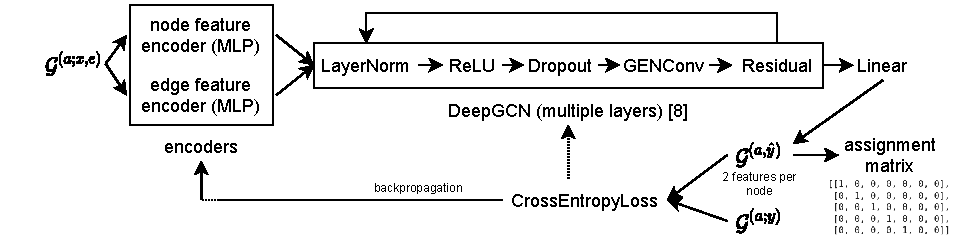
\includegraphics[width=\linewidth]{figures/nn.pdf}
			\caption{The GNN structure. For a given input graph, the node and edge features are encoded by MLPs. The resulting graph is then convolved multiple times following DeepGCN \cite{li_deepergcn_2020}. A final linear layer maps the encoded node features down to two, and CrossEntropyLoss is computed for backpropagation. For evaluation, the node features of $\G^{(a;\hat y)}$ can be reduced and reshaped to build an assignment matrix.}
			\label{fig:nn}
		\end{figure*}


\section{Results}

	This section discusses performance on the models trained with the constructed graphs, as described in \shortautoref{sec:data_preprocessing}. All models are trained with the Adam optimizer with varible exponentially decaying learning rate, adjusted manually depending on the batch size used. Unless specified otherwise, all layers use dropout (if it applies) during training with probability parameter $0.1$. The random seed is fixed at the start of each training session. Training and validation datasets are shuffled at each epoch, and make up $80\%$ and $20\%$ of the total dataset respectively.

	For evaluation, models predicting assignment matrix $\hat A$ are compared to the ground truth $A$ using the accuracy metric defined as
	$$
		\textrm{acc}(\hat A, A) = \frac{1}{n_1 n_2} \sum_{i,j} \delta_{A_{i,j}, \hat{A}_{i,j}}.
	$$

	\subsection{MLP baseline}

		As a baseline for the GNN, we train a MLP on the node features $\vec{X}$ of $G^{(a;x,e)}$ to evaluate if the graph structure (that is, addition of edge features) really adds valuable information for learning.

		For this, we need to equilibrate the labels $\vec{y}$, because asymptotically the number of nodes in the assignment graph grows as $n_1 n_2$, but the number of assignments where $y=1$ grows as $n_1$. Therefore, labels $y=1$ are underrepresented in large graphs, and equilibration is done by removing samples where $y=0$ from the training batch, until both classes are equally represented.

		Furthermore, batch normalization is applied before the MLP in order to improve training, as described in \cite{ioffe_batch_2015}.

		A hyperparameter scan was performed on the number of MLP layers and hidden channels, and found that the best performing MLP obtained an accuracy of approximately $0.88$. More layers and hidden channels were found to marginally improve the accuracy, before it started to drop due to overfitting.

	\subsection{GNN performance}

		We perform a scan on the following hyperparameters : $N_\textrm{enc}$ number of layers in both encoder MLPs, $N_\textrm{conv}$ number of DeepGCN layers, and $N_\textrm{dim}$ the number of hidden channels. Other hyperparameters, such as dropout, learning rate, exponential learning rate decay and training batch size were found to not significatively improve final performance, but can decrease training time if correctly chosen (here they were set to $0.1$, $\sim 10^{-4}$, $\sim 0.98$, $\sim 32$ respectively). For the study, we chose $N_\textrm{enc} \in \{1,2,3,4,5\}$, $N_\textrm{conv} \in \{1,2,3,4,5,8,11\}$ and $N_\textrm{dim} \in \{30, 60, 90, 120\}$. \shortautoref{fig:hparams} plots the results of the hyperparameter scan in parallel coordinates.

		Models with less than $0.99$ accuracy are obtained with few parameters overall, $N_\textrm{enc} \in \{1,2,3\}$, $N_\textrm{conv} \in \{1,2,3,4\}$ and $N_\textrm{dim} \in \{30, 60\}$. For better accuracy, it was found most effective to increase the number of encoder layers $N_\textrm{enc} \in \{2,3\}$, which systematically drove up the accuracy up to $0.999$. Following this, increasing $N_\textrm{enc}$ only marginally improved accuracy, but allowing up to 5 convolution layers gave models obtaining accuracy of up to $0.9999$. In this regime, the graph neural network is able to capture most of the complexity of the problem, but still struggles with edge cases (for instance, a cell moving a large amount). Further increasing the number of parameters (via $N_\textrm{conv}$ or $N_\textrm{dim}$, they seem to compensate each other) results in even better accuracy, where edge cases are now correctly handled. The best models obtained an accuracy of $0.99997$, and utilized $N_\textrm{enc} \geq 3$, $N_\textrm{conv} \geq 8$ and $N_\textrm{dim} \geq 80$.

		Intuitively, the performance gain of increasing $N_\textrm{enc}$ eventually caps off, because each cell graph node or edge is decribed with only 3 features, and the MLP can only transform information it is given. Increasing $N_\textrm{conv}$ intuitively can be seen as increasing the ``communication distance'' between cells, meaning each node has a ``better view'' of the whole graph structure. This of course comes with the cost of requiring more dimensions to store the information in, explaining the need to increase $N_\textrm{dim}$, and how both compensate each other. It is not useful to be able to ``see'' further in the graph ($N_\textrm{conv}$ large) if you cannot ``store'' the information ($N_\textrm{dim}$ small), and vice-versa.

		We now compare the performance of the best GNN model ($N_\textrm{enc}=5$, $N_\textrm{conv}=11$, $N_\textrm{dim}=120$) against the built-in tracking system of YeaZ, using the test dataset. From the 180 frames in the dataset, 885 pairs are tested, corresponding to frames separated by 5 to 25 minutes. Numerical results are presented in \shortautoref{tab:test_acc}. The linear sum assignment method works the best, and performs better than YeaZ, especially for pairs of frames separated by a long time difference, and in situations where cells move around a lot (specific examples are shown in \shortautoref{fig:mistracks}). The dataset's frames were separated by 5 minutes here, however one should expect approximately 15 minutes of frame separation in real applications, in which case this method has been shown to be performant.

		% Out of the 180 interframes of the testing set, YeaZ's tracker made at least one mistake on 3 of them, while our model made none. This seems plausible, as this test evaluates performance on only one frame difference (5 minutes), but the GNN has been trained on frames separated by at most  Accuracies for different methods of generating assignment matrice from the model's output are reported in \shortautoref{tab:test_acc}. This of course is not enough testing data to definitely conclude

		% Note that experimentally, better tracking performance has been observed when using values larger than this threshold, around $2 \nunit{\micro \meter}$. This of course depends on the exact colony morphology

		\begin{table}
			\centering
			% \begin{tabular}{l||rrrrr|r}
			% 	\toprule
			% 	{} &       naive &     fw &    bw &  bw+corr &      linsum &        yeaz \\
			% 	\midrule
			% 	mean  &    0.98698 &    0.99834 &    0.98689 &       0.99534 &    \textbf{0.99991} &    0.99420 \\
			% 	std   &    0.04319 &    0.01482 &    0.04011 &       0.01767 &    0.00064 &    0.05908 \\
			% 	min   &    0.77777 &    0.77777 &    0.75000 &       0.77777 &    0.99259 &    0.33333 \\
			% 	25\%   &    0.99725 &    1.00000 &    0.99359 &       1.00000 &    1.00000 &    1.00000 \\
			% 	50\%   &    1.00000 &    1.00000 &    1.00000 &       1.00000 &    1.00000 &    1.00000 \\
			% 	75\%   &    1.00000 &    1.00000 &    1.00000 &       1.00000 &    1.00000 &    1.00000 \\
			% 	max   &    1.00000 &    1.00000 &    1.00000 &       1.00000 &    1.00000 &    1.00000 \\
			% 	\bottomrule
			% \end{tabular}
			\begin{tabular}{lrrrrrrrr}
			\toprule
			{} &             mean &       std &      25\% &  50\% &  75\% \\
			\midrule
			naive         &  0.986984 &  0.043199 &  0.997253 &  1.0 &  1.0 \\
			fw            &  0.998341 &  0.014823 &  1.000000 &  1.0 &  1.0 \\
			bw            &  0.986895 &  0.040118 &  0.993590 &  1.0 &  1.0 \\
			bw+corr       &  0.995342 &  0.017675 &  1.000000 &  1.0 &  1.0 \\
			linsum        &  \textbf{0.999913} &  0.000645 &  1.000000 &  1.0 &  1.0 \\
			\midrule
			yeaz          &  0.994201 &  0.059083 &  1.000000 &  1.0 &  1.0 \\
			\bottomrule
			\end{tabular}
			\caption{Test accuracy of different methods of generating the assignment matrices from the GNN's output. The testing set (\texttt{colony007}) was split into pairs of 885 interframes, separated in real time by 5 to 25 minutes. ``naive'' refers to classifying each node simply based on the weights for each class. ``fw'' refers to the forward method, which forces each cell in the first frame to match one in the second frame. ``bw'' refers to the backwards method, which forces each cell in the second frame to match one in the first frame. ``bw+corr'' is a corrected version of the backward method, which accounts for buds. ``linsum'' uses the linear sum optimization method, as presented in \shortautoref{sec:methods:pred}. ``yeaz'' is the baseline tracking method. See \texttt{experiment\_gnn/pipeline.ipynb} for more information.}
			\label{tab:test_acc}
		\end{table}


\section{Conclusion}

	We have shown that this graph neural network model is able to learn the structure of a yeast cell colony, and is able to reliably track cells from frame to frame. It has been shown that the model exceeds YeaZ's integrated tracker performance, using a relatively small training dataset of only 4 colonies growing over 15 hours and imaged every 5 minutes. If implemented in YeaZ's GUI, tracking tasks will become easier and significantly less time-consuming, especially for large colonies.

	One of the limitations of this model is the need to have segmented the images and verified the segmentations. We however argue that thanks to advancements in this domain \cite{dietler_convolutional_2020,stringer_cellpose_2020}, this has become a trivial task. Nevertheless, it is a good practice to verify the segmentations manually, and correct as needed.

	The model presented in this report essentially only uses two graphs as an input, and could benefit from having a ``longer history'' of the colony in order to make better tracking predictions. Multiple papers \cite{singer_node_2019,jin_recurrent_2020,rossi_temporal_2020} address the problem of temporal graphs, and it might be worth investigating to further the research. In summary, using temporal graph networks are a promising approach to constructing lineages from only phase contrast (or bright field) microscopy movies. This would likely have to be coupled to an attention system, for which literature and implementations for graph neural networks already exist \cite{velickovic_graph_2018,brody_how_2021}.

	% Rome wasn't built in a day, and graph neural networks aren't mastered in a month.

\newpage
\bibliographystyle{IEEEtran}
\bibliography{literature}

\newpage
\appendix

	\begin{figure}[h!]
		\centering
		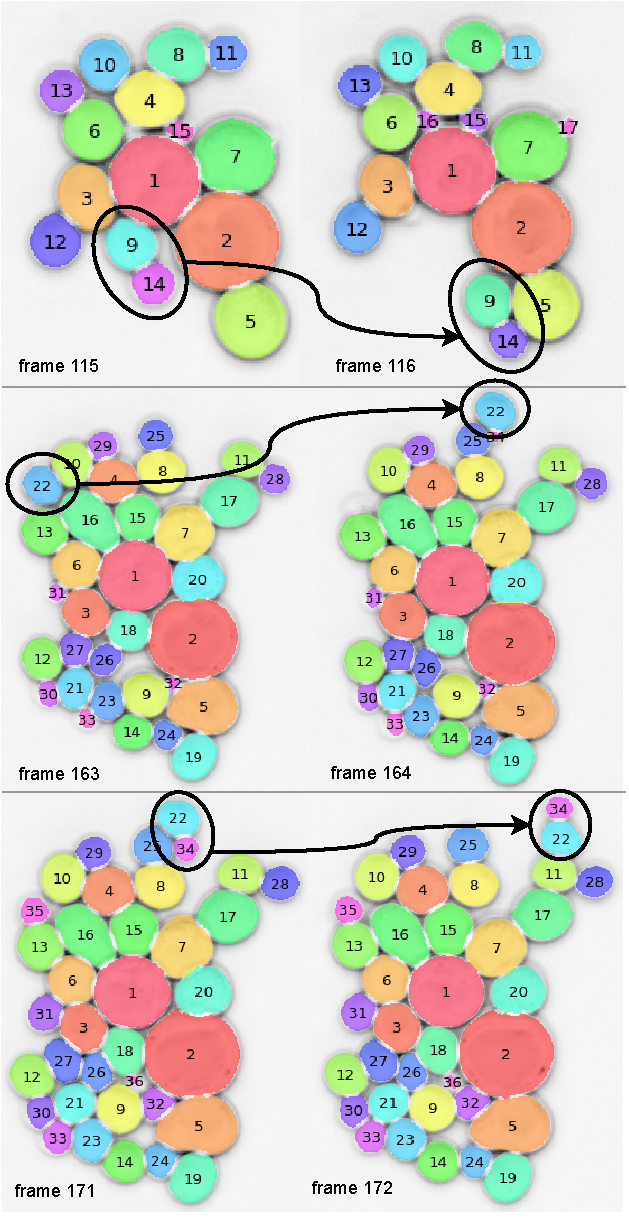
\includegraphics[width=\linewidth]{figures/mistracks.pdf}
		\caption{Segmentations from \texttt{colony007} highlighting moving cells. Out of the 179 interframes, YeaZ makes 3 tracking mistakes. On frame 115, cells 9 and 14 move together towards cell 5, and YeaZ tracks cell 9 to cell 16 and cell 14 to cell 9. On frame 163, cell 22 moves around the top of the colony, and YeaZ tracks cell 10 to 22, cell 10 to 29, cell 29 to cell 25 and cell 25 to 34. On frame 171, cells 22 and 34 move together around the top while swapping places, and YeaZ tracks cell 22 to 34 and vice-versa.}
		\label{fig:mistracks}
	\end{figure}

	\begin{figure}
		\centering
		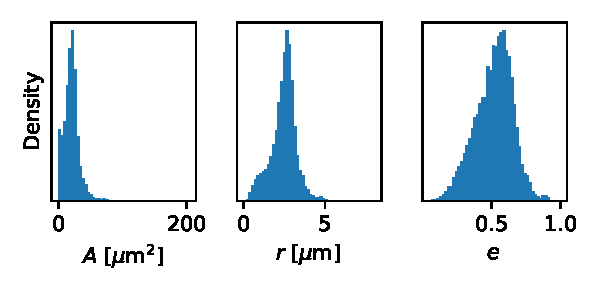
\includegraphics[width=\linewidth]{figures/hist_x.pdf}
		\captionof{figure}{Distribution of node features.}
		\label{fig:hist_x}
	\end{figure}

	\begin{figure}
		\centering
		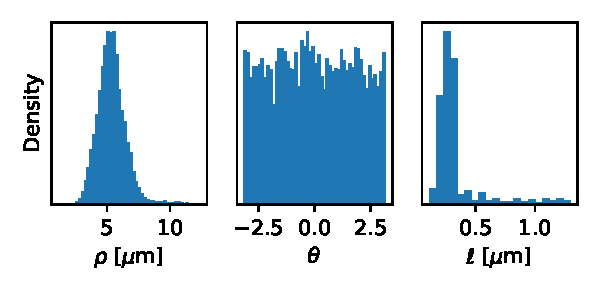
\includegraphics[width=\linewidth]{figures/hist_e.pdf}
		\captionof{figure}{Distribution of edge features.}
		\label{fig:hist_e}
	\end{figure}

	\begin{figure}
		\centering
		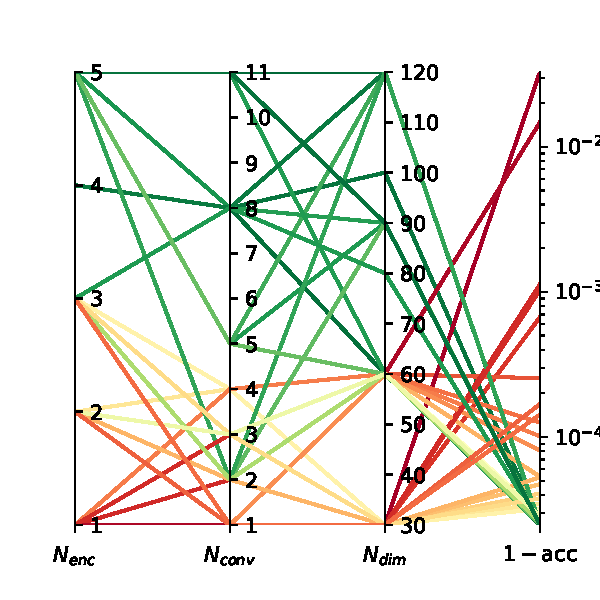
\includegraphics[width=\linewidth]{figures/hparams.pdf}
		\caption{Parallel coordinates plot of the hyperparameter scan. The best performing model uses $N_\textrm{enc}=5$, $N_\textrm{conv}=11$, $N_\textrm{dim}=120$, but a very similar performance can be achieved for less parameters, $N_\textrm{enc} \geq 3$, $N_\textrm{conv} \geq 8$ and $N_\textrm{dim} \geq 80$.}
		\label{fig:hparams}
	\end{figure}

\end{document}
